
% $Header: /cvsroot/latex-beamer/latex-beamer/solutions/generic-talks/generic-ornate-15min-45min.en.tex,v 1.5 2007/01/28 20:48:23 tantau Exp $

\documentclass[smaller]{beamer}
\mode<presentation>
{
  \usetheme{Singapore}
  \usefonttheme[onlymath]{serif}
  % or ...
 %  \setbeamercovered{transparent}
  % or whatever (possibly just delete it)
}


\usepackage[czech]{babel}
% or whatever
\usepackage[utf8]{inputenc}
% or whatever
%\usepackage{times}
%\usepackage[T1]{fontenc}
% Or whatever. Note that the encoding and the font should match. If T1
% does not look nice, try deleting the line with the fontenc.


\title{PAS04 - Spojitá rozdělení a náhodné vektory}

\author{Jan B\v rezina}
\institute % (optional, but mostly needed)
{
  %\inst{2}%
  Technical University of Liberec
}


% If you wish to uncover everything in a step-wise fashion, uncomment
% the following command: 

%\beamerdefaultoverlayspecification{<+->}

% ***************************************** SYMBOLS
\def\div{{\rm div}}
\def\Lapl{\Delta}
\def\grad{\nabla}
\def\supp{{\rm supp}}
\def\dist{{\rm dist}}
%\def\chset{\mathbbm{1}}
\def\chset{1}

\def\Tr{{\rm Tr}}
\def\sgn{{\rm sgn}}
\def\to{\rightarrow}
\def\weakto{\rightharpoonup}
\def\imbed{\hookrightarrow}
\def\cimbed{\subset\subset}
\def\range{{\mathcal R}}
\def\leprox{\lesssim}
\def\argdot{{\hspace{0.18em}\cdot\hspace{0.18em}}}
\def\Distr{{\mathcal D}}
\def\calK{{\mathcal K}}
\def\FromTo{|\rightarrow}
\def\convol{\star}
\def\impl{\Rightarrow}
\DeclareMathOperator*{\esslim}{esslim}
\DeclareMathOperator*{\esssup}{ess\,sup}
\DeclareMathOperator{\ess}{ess}
\DeclareMathOperator{\osc}{osc}
\DeclareMathOperator{\curl}{curl}

%\def\Ess{{\rm ess}}
%\def\Exp{{\rm exp}}
%\def\Implies{\Longrightarrow}
%\def\Equiv{\Longleftrightarrow}
% ****************************************** GENERAL MATH NOTATION
\def\Real{{\rm\bf R}}
\def\Rd{{{\rm\bf R}^{\rm 3}}}
\def\RN{{{\rm\bf R}^N}}
\def\D{{\mathbb D}}
\def\Nnum{{\mathbb N}}
\def\Measures{{\mathcal M}}
\def\d{\,{\rm d}}               % differential
\def\sdodt{\genfrac{}{}{}{1}{\rm d}{{\rm d}t}}
\def\dodt{\genfrac{}{}{}{}{\rm d}{{\rm d}t}}

\def\vc#1{\mathbf{\boldsymbol{#1}}}     % vector
\def\tn#1{{\mathbb{#1}}}    % tensor
\def\abs#1{\lvert#1\rvert}
\def\Abs#1{\bigl\lvert#1\bigr\rvert}
\def\bigabs#1{\bigl\lvert#1\bigr\rvert}
\def\Bigabs#1{\Big\lvert#1\Big\rvert}
\def\ABS#1{\left\lvert#1\right\rvert}
\def\norm#1{\bigl\Vert#1\bigr\Vert} %norm
\def\close#1{\overline{#1}}
\def\inter#1{#1^\circ}
\def\ol#1{\overline{#1}}
\def\ul#1{\underline{#1}}
\def\eqdef{\mathrel{\mathop:}=}     % defining equivalence
\def\where{\,|\,}                    % "where" separator in set's defs
\def\timeD#1{\dot{\overline{{#1}}}}

% ******************************************* USEFULL MACROS
\def\RomanEnum{\renewcommand{\labelenumi}{\rm (\roman{enumi})}}   % enumerate by roman numbers
\def\rf#1{(\ref{#1})}                                             % ref. shortcut
\def\prtl{\partial}                                        % partial deriv.
\def\Names#1{{\scshape #1}}
\def\rem#1{{\parskip=0cm\par!! {\sl\small #1} !!}}

\def\Xint#1{\mathchoice
{\XXint\displaystyle\textstyle{#1}}%
{\XXint\textstyle\scriptstyle{#1}}%
{\XXint\scriptstyle\scriptscriptstyle{#1}}%
{\XXint\scriptscriptstyle\scriptscriptstyle{#1}}%
\!\int}
\def\XXint#1#2#3{{\setbox0=\hbox{$#1{#2#3}{\int}$}
\vcenter{\hbox{$#2#3$}}\kern-.5\wd0}}
\def\ddashint{\Xint=}
\def\dashint{\Xint-}

% ******************************************* DOCUMENT NOTATIONS
% document specific
\def\rh{\varrho}
\def\vl{{\vc{u}}}
\def\th{\vartheta}
\def\vx{\vc{x}}
\def\vX{\vc{X}}
\def\vr{\vc{r}}
\def\veta{\vc{\eta}}
\def\dx{\,\d\vx}
\def\dt{\,\d t}
\def\bulk{\zeta}
\def\cS{\close{S}}
\def\eps{\varepsilon}
\def\phi{\varphi}
\def\Bog{{\mathcal B}}
\def\Riesz{{\mathcal R}}
\def\distr{\mathcal D}
\def\Item{$\bullet$}

\def\MEtst{\mathcal T}
%***************************************************************************
\setbeamercolor{my blue}{fg=blue}
\def\blue#1{{\usebeamercolor[fg]{my blue} #1}}
\setbeamercolor{my green}{fg=green}
\def\green#1{{\usebeamercolor[fg]{my green} #1}}
\setbeamercolor{my red}{fg=red}
\def\red#1{{\usebeamercolor[fg]{my red} #1}}
\def\xskip{{\vspace{2ex}}}

\begin{document}

\begin{frame}
  \titlepage
\end{frame}

% zvýraznění definovaného pojmu
\def\df{\usebeamercolor[fg]{my red}\it}

\section{Spojité náhodné veličiny}
\begin{frame}{Rovnoměrné rozdělení $R(a,b)$}

hustota: 
\[f(x) = \left\{
   \begin{array}{l}
    \frac{1}{b-a}  \qquad \text{pro }x\in[a,b]\\
     0 \qquad \text{jinde}
   \end{array}
\right.
\]
odvození \dots\\

distribuční funkce: 
\[f(x) = \left\{
   \begin{array}{l}
    0 \qquad \text{pro } x< a\\
    \frac{x-a}{b-a}  \qquad \text{pro }x\in[a,b]\\
     1 \qquad \text{pro } x> b
   \end{array}
\right.
\]
střední hodnota:
\[
 EX = \int_a^b \frac{x}{b-a} \dx = \frac{1}{2(b-a)} \big(b^2 - a^2\big) = \frac{a+b}{2}
\]
rozptyl (trochu delší počítáni):
\[
 DX = \int_a^b =\frac{(a-b)^2}{12}
\]
\end{frame}

\begin{frame}{Vlastnosti rovnoměrného rozdělení.}
\begin{theorem}
Pro libovolnou n. v. $X$ se spojitou rostoucí distribuční funkcí $F_X$ má veličina 
\[
  Y=F_X(X)
\]
rovnoměrné rozdělení $R(0,1)$. Značíme: $Y \sim R(0,1)$
\end{theorem}
a podobně opačně:
\begin{theorem}
Nechť n.v. $Y \sim R(0,1)$ a $F$ je nějká distribuční funkce, pak $X = F_X^{-1}(Y)$ je náhodná veličina s distribuční funkcí $F_X=F$.
\end{theorem}
\begin{itemize}
\item Ve druhé větě je $F$ libovolná distribuční funkce, spojitá i nespojitá. 
\item Počítačové generátory (pseudo)náhodných čísel obvykle generují čísla s rozdělením $R(0,1)$.
\item Druhou větu pak lze použít ke generování náhodných čísel předepsaného rozdělení. (v praxi spíše specializované aproximace)
\end{itemize}

\end{frame}

\begin{frame}{Exponenciální rozdělení $E(\lambda)$}
$X$ je doba do poruchy při Poissonově procesu s hustotou $\lambda$. Odvození:
\vspace{2ex}
Uvažme náhodnou veličinu $N_t \sim Po(\lambda, t)$.\\
Jevy $\{X<t\}$ (doba do poruchy je menší než $t$ 
a $\{N_t \ge 1\}$ (za dobu $t$ nastane alespoň jedna porucha) jsou identické.\\
\[
 F_X(t)=P(X<t) = 1 - P(N_t <1) = 1 - \frac{(\lambda t)^0 e^{-\lambda t}}{0!} = 1 - e^{-\lambda t}
\]
\[
  f_X(t) = \frac{d}{dt} F_X(t) = \lambda e^{-\lambda t}
\]
v obou případech pro $t>0$, jelikož doba musí být kladná.
\[
 EX = \int_0^\infty t\lambda e^{-\lambda t} \d t 
 = \Big[te^{-\lambda t}\Big]_0^{\infty} - \int_0^\infty e^{-\lambda t}
 = \frac{1}{\lambda}
\]
\[
 DX = \frac{1}{\lambda^2}
\]
\end{frame}

\begin{frame}{Exponenciální rozdělení - bez paměti}
Doba do poruchy je nezávislá na historii poruch:
Pravděpodobnost, že nenastane porucha do času $a+b$ za podmínky, že nenastala do
času $a$ je stejná jako pravděpodobnost, že porucha nenastane do času $b$
\begin{multline*}
 P(X > a+b | X>a) = \frac{1-F(a+b)}{1-F(a)} \\
= \frac{e^{a+b}}{e^a} = e^b = 1 - F(b) = P(X>b)
\end{multline*}

\end{frame}


\begin{frame}{Erlangovo rozdělení $Erlang(k,\lambda)$}
$X$ je doba do $k$-té poruchy při Poissonově procesu s hustotou $\lambda$. 
Speciální případ tzv. \red{Gamma rozdělení} pro $k$ celočíselné.
\[
 f_X(t)=\lambda e^{-\lambda t} \frac{(\lambda t)^{k-1}}{(k-1)!}
\]
\[
  F_X(t) = 1- e^{-\lambda t}\sum_{i=0}^{k-1} \frac{(\lambda t)^{i}}{i!}
\]
\[
 EX = \frac{k}{\lambda}
\]
\[
 DX = \frac{k}{\lambda^2}
\]

\end{frame}

\begin{frame}{Vztah Bernoulliho pokusů a Poissonova procesu}
 \begin{center}
 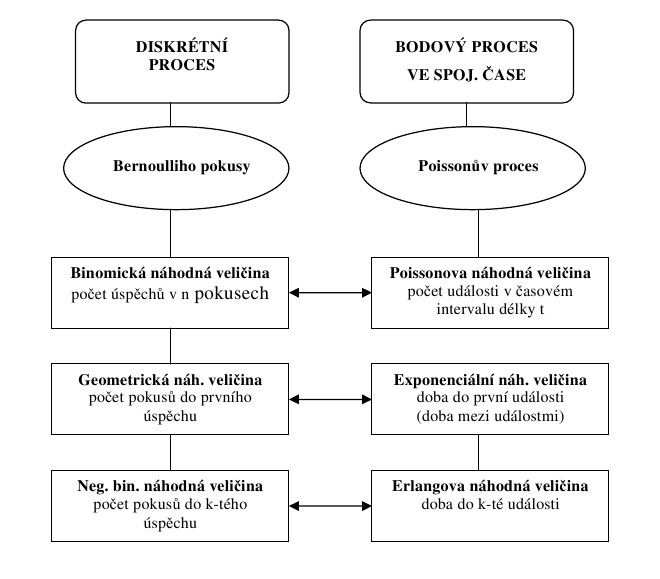
\includegraphics[scale=0.5]{./bernoulli_poisson.png}
 % bernoulli_poisson.png: 660x579 pixel, 96dpi, 17.46x15.32 cm, bb=0 0 495 434
\end{center}
\end{frame}

\begin{frame}{Weibullovo rozdělení $W(\Theta, \beta)$}
Doba do poruchy s ohledem na období doby života.

\[
 F_X(t) = 1-exp\big( -(t/\Theta)^\beta \big )
\]
\dots podobnost s exponenciálním rozdělením.
\end{frame}

\begin{frame}{Weibullovo rozdělení - vliv arametru $\beta$}
vliv parametru tvaru $\beta$ na intenziu poruch:
 \begin{center}
 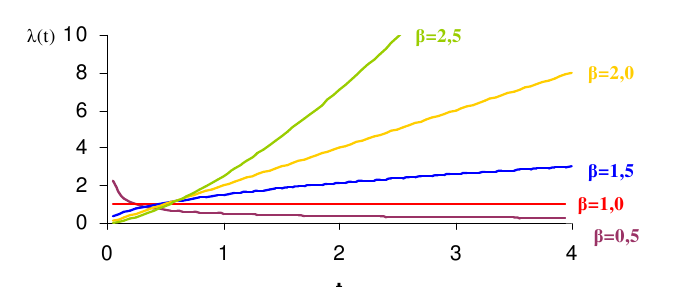
\includegraphics[scale=0.5]{./weibull_intenzita.png}
\end{center}
\begin{center}
 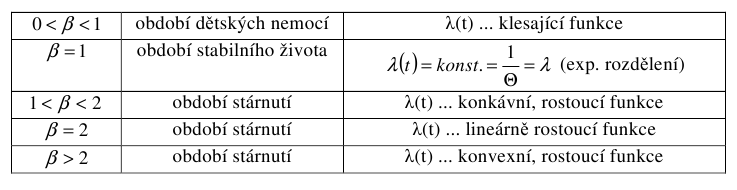
\includegraphics[scale=0.5]{./weibull_shape.png}
\end{center}
\end{frame}

\begin{frame}{Normální rozdělení $N(\mu, \sigma^2)$}
Součet velkého množství nezávislých NV. Přírodní jevy.\\
hustota:
\[
 f(x) = \frac{1}{\sqrt{2\pi \sigma^2}} exp\Big( - \frac{ (x - \mu)^2}{2\sigma^2} \Big)
\]
distribuční funkce: \dots integrálem z hustoty\\
\vspace{2ex}
$EX = \mu$\\
$DX = \sigma^2$

\end{frame}


\begin{frame}{Normované normální rozdělení $N(0,1)$}
Standardizace normální náhodné veičiny $X \sim N(\mu, \sigma^2)$:
\[
 Y = \frac{X - \mu}{\sigma} \quad \sim N(0,1)
\]
a naopak \dots
\end{frame}

\begin{frame}{Ověření normality}

\end{frame}


\begin{frame}{Log-normální rozdělení $LN(\mu, \sigma^2)$}
\end{frame}

\section{Náhodný vektor}

\begin{frame}{Sdružená distribuční funkce}
\end{frame}

\begin{frame}{Hustota pravděpodobnosti}
\end{frame}

\begin{frame}{Marginální rozdělení pravděpodobnosti}
\end{frame}

\begin{frame}{Nezávislost}
\end{frame}

\begin{frame}{Podmíněné rozdělení}
\end{frame}

\begin{frame}{Charakteristiky}
\end{frame}

\begin{frame}{Kovariance, korelace, korelační matice}
\[
  {\rm cov}(X,Y) = E(X-EX)(Y-EY)
\]
\[
  {\rm corr}(X,Y) = \frac{cov(X,Y)}{\sigma(X)\sigma(Y)}
\]
\[
  ({\rm var} \vc X )_{i,j}=cov(X_i,X_j)  
\]



 

\end{frame}


\begin{frame}{Dvourozměrné normální rozdělení}
\end{frame}

\begin{frame}{Multinomické rozdělení}
\end{frame}


\end{document}


